\chapter{Genomas de células e de vírus}\label{ch:b1:genomes}

Dois metros de \omterm{def:b1:nucleic-acids:chain}{DNA} estão dobrados dentro de um núcleo de seis
micrômetros de diâmetro, e dobrados de tal modo que qualquer um de vinte
mil \omterm{def:b1:genomes:gene}{genes} pode ser encontrado e lido em poucos minutos. Uma bactéria
dobra um milímetro e meio numa \omterm{def:b1:cell-unit-of-life:cell}{célula} mil vezes menor, e o copia a cada
vinte minutos. Um \omterm{def:b1:genomes:virus}{vírus} carrega alguns milhares de letras numa casca de
\omterm{def:b1:proteins:peptide}{proteína} e as lê com uma \omterm{def:b1:cell-unit-of-life:cell}{célula} que não é dele. Este capítulo descreve o
\emph{\omterm{def:b1:genomes:genome}{genoma}} --- o conjunto do \omterm{def:b1:nucleic-acids:chain}{DNA} de um \omterm{def:b1:organism-environment:organism}{organismo} --- como objeto
físico: como o \omterm{def:b1:nucleic-acids:chain}{DNA} das bactérias, das \omterm{def:b1:cell-unit-of-life:prokeuk}{células eucarióticas}, das
\omterm{def:b1:cell-unit-of-life:prokeuk}{organelas} e dos \omterm{def:b1:genomes:virus}{vírus} é organizado, o que ele contém além dos \omterm{def:b1:genomes:gene}{genes}, e
por que a quantidade dele diz tão pouco sobre o \omterm{def:b1:organism-environment:organism}{organismo} que o carrega.

\section{O genoma bacteriano}

\begin{definition}[Genoma, cromossomo, nucleoide]\label{def:b1:genomes:genome}
O \emph{genoma}\index{genoma} de uma \omterm{def:b1:cell-unit-of-life:cell}{célula} é a totalidade do \omterm{def:b1:nucleic-acids:chain}{DNA} dela:
a informação para cada \omterm{def:b1:proteins:peptide}{proteína} e cada \omterm{def:b1:nucleic-acids:chain}{RNA} que ela consegue fabricar, e
as sequências que controlam quando eles são fabricados. Um
\emph{cromossomo}\index{cromossomo} é uma molécula de \omterm{def:b1:nucleic-acids:chain}{DNA} com as
\omterm{def:b1:proteins:peptide}{proteínas} que a organizam. Uma bactéria em geral tem um só, circular, de
um a dez milhões de \omterm{thm:b1:nucleic-acids:helix}{pares de bases} (a \emph{E. coli}: $\num{4.6e6}$,
\qty{1.5}{mm} de comprimento), dobrado numa região do \omterm{def:b1:cell-unit-of-life:cell}{citoplasma}, o
\emph{nucleoide}\index{nucleoide}, sem membrana em volta. Além do
cromossomo, muitas bactérias carregam
\emph{plasmídeos}\index{plasmídeo}: círculos pequenos, de alguns
milhares a algumas centenas de milhares de pares, em uma a centenas de
cópias, que se replicam por conta própria e carregam \omterm{def:b1:genomes:gene}{genes} opcionais ---
resistência a antibióticos, toxinas, a maquinaria para se transferirem a
outra \omterm{def:b1:cell-unit-of-life:cell}{célula}.
\end{definition}

\begin{proposition}[Como uma bactéria dobra o cromossomo dela]\label{prop:b1:genomes:supercoiling}
\index{superenrolamento}
Um \omterm{def:b1:nucleic-acids:chain}{DNA} circular cujas extremidades não podem girar pode ser torcido como
um elástico: é o \emph{superenrolamento}. \omterm{def:b1:enzymes:enzyme}{Enzimas} chamadas
\emph{topoisomerases} cortam, passam e reselam as fitas para acrescentar
ou remover voltas; a \emph{girase} usa \omterm{def:b1:water-small-molecules:atp}{ATP} para introduzir super-hélices
negativas, que desenrolam a hélice e a tornam ao mesmo tempo mais
compacta e mais fácil de abrir. O \omterm{def:b1:genomes:genome}{cromossomo} da \emph{E. coli} é
organizado em umas cinquenta alças, cada uma superenrolada de forma
independente e ancorada num eixo proteico, de modo que os \qty{1.5}{mm}
ocupam um \omterm{def:b1:genomes:genome}{nucleoide} de cerca de um micrômetro --- uma compactação de mil
vezes --- e ao mesmo tempo qualquer alça pode ser desenrolada para
leitura ou cópia sem perturbar as demais. Pequenas \omterm{def:b1:proteins:peptide}{proteínas} básicas
(semelhantes a \omterm{def:b1:genomes:nucleosome}{histonas}, embora não aparentadas a elas) dobram e
interligam o \omterm{def:b1:nucleic-acids:chain}{DNA} por toda parte.
\end{proposition}

\begin{omfigure}
\begin{tikzpicture}[font=\footnotesize, line cap=round]
  % relaxed circle
  \draw[very thick, omDef] (0,0) circle (1.1);
  \node[anchor=north, align=center] at (0,-1.35) {círculo relaxado\\ (10.5 pb por volta)};
  % supercoiled: figure-eight / plectoneme
  \draw[very thick, omDef, domain=0:360, samples=240, smooth, variable=\t] plot ({4.3+1.05*cos(\t)}, {0.32*sin(4*\t)});
  \node[anchor=north, align=center] at (4.3,-1.35) {superenrolado negativamente:\\ desenrolado, compacto};
  \draw[->, thick] (1.35,0.15) -- (3.1,0.15) node[midway, above, align=center] {girase (ATP)};
  \draw[->, thick] (3.1,-0.25) -- (1.35,-0.25) node[midway, below, align=center] {topoisomerase I};
  % looped nucleoid
  \fill[omProp!40] (8.7,0) circle (0.35);
  \foreach \a in {0,45,...,315} {
    \draw[very thick, omDef] (8.7,0) .. controls ({8.7+1.6*cos(\a-20)},{1.6*sin(\a-20)}) and ({8.7+1.6*cos(\a+20)},{1.6*sin(\a+20)}) .. (8.7,0);
  }
  \node[anchor=north, align=center] at (8.7,-1.35) {o nucleoide: cerca de cinquenta\\ alças superenroladas num eixo proteico};
\end{tikzpicture}

{\small Um \omterm{def:b1:genomes:genome}{cromossomo} circular relaxado, superenrolado e organizado em
alças. O superenrolamento compacta a molécula e armazena a energia que
ajuda a abri-la; as alças permitem desenrolar uma região de cada vez.}
\end{omfigure}

\begin{example}[Um genoma denso]\label{ex:b1:genomes:dense}
Dos \qty{4.6}{Mb} do \omterm{def:b1:genomes:genome}{cromossomo} da \emph{E. coli}, \qty{88}{\%}
codificam \omterm{def:b1:proteins:peptide}{proteína}: uns \num{4300} \omterm{def:b1:genomes:gene}{genes} de cerca de \num{1000} pares
cada, encaixados um atrás do outro com uma centena de pares entre eles,
muitos agrupados em \emph{óperons} transcritos juntos
(\cref{ch:b1:expression-control}). Um \omterm{def:b1:genomes:genome}{plasmídeo} de \qty{5}{kb} pode
carregar três \omterm{def:b1:genomes:gene}{genes} e existir em cinquenta cópias; o \omterm{def:b1:genomes:gene}{gene} de
resistência que ele carrega pode se espalhar pelas bactérias de uma ala
de hospital em poucas semanas, por conjugação, mais rápido do que
qualquer mutação poderia surgir.
\end{example}

\section{O genoma eucariótico: a cromatina}

\begin{definition}[Nucleossomo, cromatina]\label{def:b1:genomes:nucleosome}
\index{nucleossomo}\index{histona}\index{cromatina}
Num núcleo eucariótico o \omterm{def:b1:nucleic-acids:chain}{DNA} está enrolado em \omterm{def:b1:proteins:peptide}{proteínas}: \qty{147}{}
\omterm{thm:b1:nucleic-acids:helix}{pares de bases} dão 1.7 volta em torno de um octâmero de oito
\emph{histonas} (duas de cada uma das H2A, H2B, H3 e H4, \omterm{def:b1:proteins:peptide}{proteínas}
pequenas ricas em lisina e arginina que neutralizam os fosfatos),
formando um \emph{nucleossomo}\index{nucleossomo} de \qty{11}{nm} de
diâmetro; os nucleossomos se seguem uns aos outros a cada \qty{200}{}
pares, mais ou menos, como contas num colar, com uma quinta histona, a
H1, selando cada conta. Essa \emph{cromatina} se dobra ainda mais: numa
fibra de \qty{30}{nm}, em alças de dezenas de milhares de pares
ancoradas num arcabouço proteico e --- na divisão --- nos bastões
compactos do \omterm{def:b1:genomes:genome}{cromossomo} metafásico, dez mil vezes mais curtos que o \omterm{def:b1:nucleic-acids:chain}{DNA}
nu. A \emph{eucromatina} é a forma mais frouxa, rica em \omterm{def:b1:genomes:gene}{genes} e
transcrita da interfase; a \emph{heterocromatina}, a forma condensada e
pobre em \omterm{def:b1:genomes:gene}{genes} que permanece compacta (em torno dos \omterm{def:b1:genomes:karyotype}{centrômeros}, nas
extremidades e num \omterm{def:b1:genomes:genome}{cromossomo} X desligado).
\end{definition}

\begin{omfigure}
\begin{tikzpicture}[font=\footnotesize, >=Stealth, line cap=round]
  % level 1: double helix line
  \draw[very thick, omDef] (0,5.4) -- (3.2,5.4);
  \node[anchor=west, align=left] at (3.5,5.4) {dupla-hélice, \qty{2}{nm}};
  % level 2: beads on a string
  \draw[thick, omDef] (0,4.2) -- (3.2,4.2);
  \foreach \x in {0.4,1.2,2.0,2.8} { \fill[omProp!70] (\x,4.2) circle (0.22); \draw[thick, omDef] (\x,4.2) circle (0.3); }
  \node[anchor=west, align=left] at (3.5,4.2) {nucleossomos, \qty{11}{nm}: \qty{147}{bp} em torno de um octâmero de histonas,\\ a cada \qty{200}{bp} --- compactação $\times 6$};
  % level 3: 30 nm fibre (zigzag stack)
  \foreach \i in {0,...,9} { \fill[omProp!70] (0.2+0.3*\i,{3.0+0.18*(-1)^\i}) circle (0.17); }
  \node[anchor=west, align=left] at (3.5,3.0) {fibra de \qty{30}{nm}: nucleossomos empilhados --- $\times 40$};
  % level 4: loops on scaffold
  \draw[very thick, gray] (0,1.5) -- (3.2,1.5);
  \foreach \x in {0.4,1.2,2.0,2.8} { \draw[thick, omProp!80!black] (\x,1.5) .. controls (\x-0.35,2.3) and (\x+0.35,2.3) .. (\x,1.5); }
  \node[anchor=west, align=left] at (3.5,1.8) {alças de \qtyrange{50}{100}{kb} num arcabouço, \qty{300}{nm} --- $\times 1000$};
  % level 5: metaphase chromosome
  \draw[very thick, omThm, fill=omThm!30, rounded corners=4pt] (0.9,-0.3) rectangle (1.4,1.0);
  \draw[very thick, omThm, fill=omThm!30, rounded corners=4pt] (1.7,-0.3) rectangle (2.2,1.0);
  \fill[omThm!60!black] (1.55,0.45) ellipse (0.45 and 0.13);
  \node[anchor=west, align=left] at (3.5,0.35) {cromossomo metafásico, \qty{1400}{nm} de largura: $\times \num{10000}$\\ (\qty{8.5}{cm} de DNA em \qty{10}{\micro m})};
\end{tikzpicture}

{\small Níveis de empacotamento do \omterm{def:b1:nucleic-acids:chain}{DNA} eucariótico, da hélice ao
\omterm{def:b1:genomes:genome}{cromossomo} metafásico. Cada nível multiplica a compactação; o conjunto
chega a dez mil.}
\end{omfigure}

\begin{omfigure}
\begin{minipage}[b]{0.46\linewidth}\centering
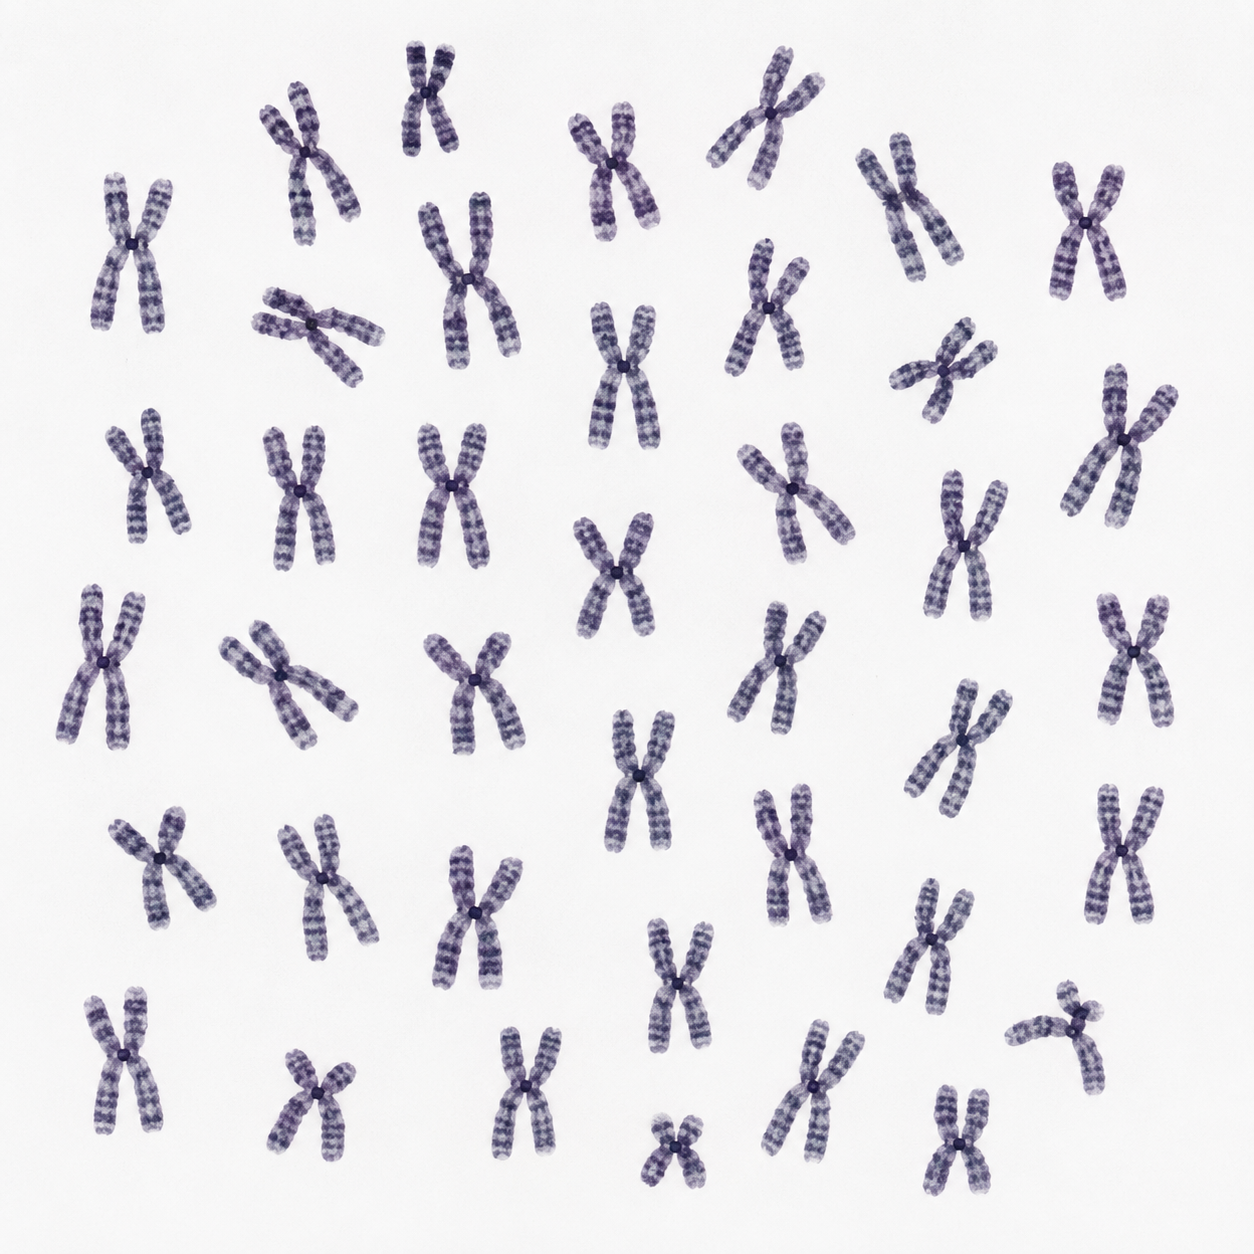
\includegraphics[width=0.94\linewidth]{images/book3/ai/b3-17-metaphase-spread.png}
\end{minipage}\hfill
\begin{minipage}[b]{0.5\linewidth}\centering
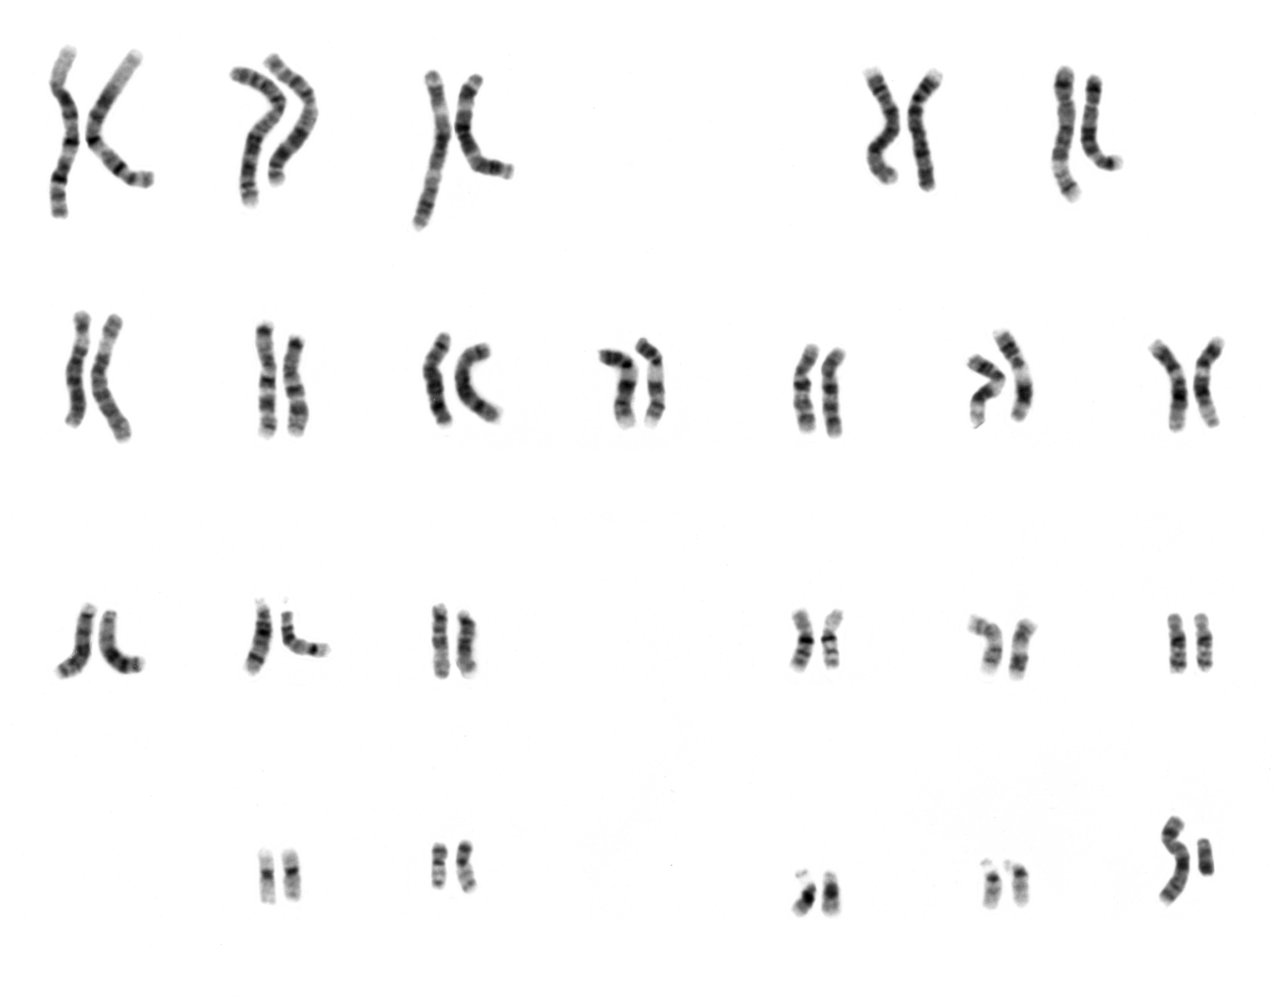
\includegraphics[width=0.96\linewidth]{images/book3/karyotype.png}
\end{minipage}

{\small À esquerda: os \omterm{def:b1:genomes:genome}{cromossomos} de uma \omterm{def:b1:cell-unit-of-life:cell}{célula} humana, espalhados a
partir de uma \omterm{def:b1:cell-unit-of-life:cell}{célula} parada na metáfase. À direita: os mesmos
\omterm{def:b1:genomes:genome}{cromossomos} ordenados por tamanho e por bandeamento num \omterm{def:b1:genomes:karyotype}{cariótipo} ---
vinte e dois pares e XY, quarenta e seis ao todo. \omterm{def:b1:genomes:karyotype}{Cariótipo}: National
Human Genome Research Institute, domínio público.}
\end{omfigure}

\begin{definition}[Cariótipo, centrômero, telômero]\label{def:b1:genomes:karyotype}
\index{cariótipo}\index{centrômero}\index{telômero}
O \emph{cariótipo} é o conjunto dos \omterm{def:b1:genomes:genome}{cromossomos} de uma \omterm{def:b1:cell-unit-of-life:cell}{célula}, ordenados
por tamanho e por padrão de bandeamento: os humanos têm 23 pares (22
autossomos e XY ou XX), $\num{6.4e9}$ \omterm{thm:b1:nucleic-acids:helix}{pares de bases} ao todo,
\qty{2.2}{m}; o maior \omterm{def:b1:genomes:genome}{cromossomo} contém \qty{250}{Mb}, e o menor
\qty{50}{}. Cada \omterm{def:b1:genomes:genome}{cromossomo} linear carrega um \emph{centrômero}, a
região estrangulada em que as duas cópias permanecem unidas depois da
replicação e em que o fuso se prende
(\cref{ch:b1:replication-mitosis}), e dois \emph{telômeros}, sequências
repetidas nas extremidades que as protegem de serem tomadas por \omterm{def:b1:nucleic-acids:chain}{DNA}
quebrado e de encurtarem a cada replicação.
\end{definition}

\begin{proposition}[O tamanho do genoma não mede a complexidade]\label{prop:b1:genomes:cvalue}
\index{paradoxo do valor C}
\begin{center}
\small
\begin{tabular}{lrr}
\hline
\omterm{def:b1:organism-environment:organism}{organismo} & \omterm{def:b1:genomes:genome}{genoma} (Mb) & \omterm{def:b1:genomes:gene}{genes} codificadores de \omterm{def:b1:proteins:peptide}{proteína} \\
\hline
\emph{E. coli} & 4.6 & \num{4300} \\
levedura & 12 & \num{6000} \\
mosca-das-frutas & 140 & \num{14000} \\
ser humano & 3200 & \num{20000} \\
milho & 2300 & \num{40000} \\
peixe pulmonado & \num{130000} & $\approx\num{20000}$ \\
\emph{Paris japonica} (um lírio) & \num{150000} & $\approx\num{30000}$ \\
\hline
\end{tabular}
\end{center}
O tamanho do \omterm{def:b1:genomes:genome}{genoma} varia mil vezes entre os eucariotos, sem relação com
o número de \omterm{def:b1:genomes:gene}{genes} nem com a complexidade do \omterm{def:b1:organism-environment:organism}{organismo} (é o
\emph{paradoxo do valor C}): um peixe pulmonado carrega quarenta vezes o
\omterm{def:b1:nucleic-acids:chain}{DNA} de um ser humano e nenhum \omterm{def:b1:genomes:gene}{gene} a mais. A diferença não está nos
\omterm{def:b1:genomes:gene}{genes}, e sim no \omterm{def:b1:nucleic-acids:chain}{DNA} entre eles.
\end{proposition}

\section{O que um genoma contém}

\begin{definition}[Anatomia de um gene]\label{def:b1:genomes:gene}
\index{gene}\index{éxon}\index{íntron}\index{promotor}
Um \emph{gene} é um trecho de \omterm{def:b1:nucleic-acids:chain}{DNA} transcrito num \omterm{def:b1:nucleic-acids:chain}{RNA} funcional --- em
geral um mensageiro para uma \omterm{def:b1:proteins:peptide}{proteína}. Um gene eucariótico codificador
de \omterm{def:b1:proteins:peptide}{proteína} compreende um \emph{promotor}, a sequência a montante em que
a transcrição começa e é controlada; os \emph{éxons}, as partes mantidas
na mensagem madura; os \emph{íntrons}, as partes transcritas e depois
recortadas (\cref{ch:b1:gene-expression}); as regiões não traduzidas de
cada extremidade da mensagem; e um terminador. Um gene humano tem em
média \qty{27}{kb} com oito éxons que somam \qty{1.5}{kb}: dezenove
vigésimos de um gene típico são íntron. Os genes bacterianos não têm
íntrons.
\end{definition}

\begin{omfigure}
\begin{tikzpicture}[font=\footnotesize, >=Stealth, line cap=round]
  \draw[very thick, gray] (0,0) -- (12.6,0);
  \fill[omExo!50] (0.2,-0.18) rectangle (1.6,0.18); \node[anchor=north] at (0.9,-0.25) {promotor};
  \fill[omDef!70] (1.6,-0.25) rectangle (2.4,0.25);
  \fill[omDef!70] (4.6,-0.25) rectangle (5.6,0.25);
  \fill[omDef!70] (8.4,-0.25) rectangle (9.0,0.25);
  \fill[omDef!70] (10.9,-0.25) rectangle (12.0,0.25);
  \node[anchor=south, omDef!70!black] at (2.0,0.3) {éxon 1};
  \node[anchor=south, omDef!70!black] at (5.1,0.3) {éxon 2};
  \node[anchor=south, omDef!70!black] at (8.7,0.3) {éxon 3};
  \node[anchor=south, omDef!70!black] at (11.45,0.3) {éxon 4};
  \node[anchor=north] at (3.5,-0.3) {íntron 1};
  \node[anchor=north] at (7.0,-0.3) {íntron 2};
  \node[anchor=north] at (9.95,-0.3) {íntron 3};
  \draw[->, thick, omExo!70!black] (1.6,0.75) -- (2.6,0.75); \node[anchor=south, font=\scriptsize] at (2.6,0.85) {a transcrição começa aqui};
  \node[anchor=north, align=center, gray] at (6.3,-0.9) {um gene humano típico: \qty{27}{kb}, dos quais \qty{1.5}{kb} de éxons;\\ os éxons são unidos no mensageiro maduro, e os íntrons descartados};
\end{tikzpicture}

{\small Um \omterm{def:b1:genomes:gene}{gene} eucariótico: um \omterm{def:b1:genomes:gene}{promotor}, \omterm{def:b1:genomes:gene}{éxons} (mantidos) alternados
com \omterm{def:b1:genomes:gene}{íntrons} (removidos depois da transcrição). Desenhado numa escala
comprimida --- num \omterm{def:b1:genomes:gene}{gene} real os \omterm{def:b1:genomes:gene}{íntrons} seriam vinte vezes mais longos
que os \omterm{def:b1:genomes:gene}{éxons}.}
\end{omfigure}

\begin{proposition}[O censo do genoma humano]\label{prop:b1:genomes:census}
\index{transpóson}\index{DNA repetido}
Dos \qty{3.2}{Gb}: cerca de \qty{1.5}{\%} codificam \omterm{def:b1:proteins:peptide}{proteína};
\qty{25}{\%} são \omterm{def:b1:genomes:gene}{íntron}; \qty{45}{\%} são os restos de
\emph{elementos transponíveis} --- sequências que se copiam para novos
lugares, quase todas há muito mortas (só o elemento Alu, de
\qty{300}{bp}, está presente em um milhão de cópias, um décimo do
\omterm{def:b1:genomes:genome}{genoma}); \qty{8}{\%} são repetições curtas em tandem (o \omterm{def:b1:nucleic-acids:chain}{DNA} satélite,
nos \omterm{def:b1:genomes:karyotype}{centrômeros} e nos \omterm{def:b1:genomes:karyotype}{telômeros}); o restante é sequência não codificante
única, que inclui os \omterm{def:b1:genomes:gene}{promotores}, os intensificadores e os \omterm{def:b1:genomes:gene}{genes} de \omterm{def:b1:nucleic-acids:chain}{RNA}
que controlam a expressão. Muitos \omterm{def:b1:genomes:gene}{genes} pertencem a \emph{famílias}
surgidas por duplicação (as globinas, os receptores olfativos --- um
milhar deles), e o \omterm{def:b1:genomes:genome}{genoma} abriga milhares de \emph{pseudogenes}, cópias
mortas que já não funcionam. Um \omterm{def:b1:genomes:genome}{genoma} não é um projeto, e sim um
registro.
\end{proposition}

\begin{omfigure}
\begin{tikzpicture}[font=\footnotesize]
  \def\R{2.1}
  % slices: coding 1.5, introns 25, transposons 45, satellite 8, other 20.5
  \fill[omThm!70] (0,0) -- (90:\R) arc (90:84.6:\R) -- cycle;
  \fill[omDef!50] (0,0) -- (84.6:\R) arc (84.6:-5.4:\R) -- cycle;
  \fill[omProp!50] (0,0) -- (-5.4:\R) arc (-5.4:-167.4:\R) -- cycle;
  \fill[omExo!50] (0,0) -- (-167.4:\R) arc (-167.4:-196.2:\R) -- cycle;
  \fill[gray!30] (0,0) -- (-196.2:\R) arc (-196.2:-270:\R) -- cycle;
  \draw[thick] (0,0) circle (\R);
  \node[anchor=west, omThm!80!black] at (0.3,2.35) {éxons codificadores \qty{1.5}{\%}};
  \draw[omThm!80!black] (87:\R) -- (0.3,2.35);
  \node[anchor=west] at (2.3,0.9) {íntrons \qty{25}{\%}};
  \node[anchor=north] at (0,-2.3) {elementos transponíveis e os restos deles \qty{45}{\%}};
  \node[anchor=east] at (-2.3,-0.4) {repetições satélite \qty{8}{\%}};
  \node[anchor=east] at (-2.3,1.2) {outro DNA único \qty{20}{\%}};
\end{tikzpicture}

{\small Do que o \omterm{def:b1:genomes:genome}{genoma} humano é feito. Os \omterm{def:b1:genomes:gene}{éxons} que codificam \omterm{def:b1:proteins:peptide}{proteína}
são uma lasca; metade do \omterm{def:b1:genomes:genome}{genoma} são os destroços de elementos que um dia
se copiaram.}
\end{omfigure}

\begin{example}[Ler o tamanho de um genoma]\label{ex:b1:genomes:sizes}
Um \omterm{def:b1:genomes:genome}{genoma} de \qty{4.6}{Mb} sem \omterm{def:b1:genomes:gene}{íntrons} e com poucas repetições contém
\num{4300} \omterm{def:b1:genomes:gene}{genes}; um de \qty{3200}{Mb} com \omterm{def:b1:genomes:gene}{íntrons} longos e metade do
comprimento em repetições contém \num{20000}; um de \qty{130000}{Mb}
contém os mesmos vinte mil. O tamanho mede quanto se acumulou no \omterm{def:b1:nucleic-acids:chain}{DNA} não
codificante de uma linhagem, e com que eficiência isso foi removido, e
não quanto o \omterm{def:b1:organism-environment:organism}{organismo} faz.
\end{example}

\section{Genomas de organelas e vírus}

\begin{definition}[Genomas de organelas]\label{def:b1:genomes:organelle}
As \omterm{def:b1:eukaryotic-cell:mitochondrion}{mitocôndrias} e os \omterm{def:b1:eukaryotic-cell:plastid}{cloroplastos} guardam um resquício do \omterm{def:b1:genomes:genome}{cromossomo} dos
ancestrais bacterianos deles (\cref{ch:b1:eukaryotic-cell}): um pequeno
círculo --- \qty{16.6}{kb} e 37 \omterm{def:b1:genomes:gene}{genes} nas \omterm{def:b1:eukaryotic-cell:mitochondrion}{mitocôndrias} humanas,
\qtyrange{120}{160}{kb} e cerca de 100 \omterm{def:b1:genomes:gene}{genes} nos \omterm{def:b1:eukaryotic-cell:plastid}{cloroplastos} --- em
muitas cópias por organela, que codifica algumas das \omterm{def:b1:proteins:peptide}{proteínas} deles e
os \omterm{def:b1:nucleic-acids:chain}{RNAs} dos ribossomos deles. As demais \omterm{def:b1:proteins:peptide}{proteínas} deles vêm de \omterm{def:b1:genomes:gene}{genes}
nucleares. Na maioria dos animais o \omterm{def:b1:genomes:genome}{genoma} mitocondrial é herdado apenas
da mãe, com o \omterm{def:b1:cell-unit-of-life:cell}{citoplasma} do óvulo.
\end{definition}

\begin{definition}[Vírus]\label{def:b1:genomes:virus}
\index{vírus}\index{capsídeo}
Um \emph{vírus} é um \omterm{def:b1:genomes:genome}{genoma} dentro de uma casca de \omterm{def:b1:proteins:peptide}{proteína}, o
\emph{capsídeo} --- às vezes envolvido por uma membrana, o
\emph{envelope}, tomada de uma \omterm{def:b1:cell-unit-of-life:cell}{célula} hospedeira ---, que só se
reproduz dentro de uma \omterm{def:b1:cell-unit-of-life:cell}{célula}, usando os ribossomos, a energia e os
precursores dela. O \omterm{def:b1:genomes:genome}{genoma} dele pode ser \omterm{def:b1:nucleic-acids:chain}{DNA} ou \omterm{def:b1:nucleic-acids:chain}{RNA}, de fita dupla ou
simples, linear ou circular, uma única molécula ou várias: de
\qty{5}{kb} (uns poucos \omterm{def:b1:genomes:gene}{genes}) a \qty{1.2}{Mb} (um milhar, nos vírus
gigantes). Fora de uma \omterm{def:b1:cell-unit-of-life:cell}{célula} um vírus nada faz: ele não é uma \omterm{def:b1:cell-unit-of-life:cell}{célula},
não tem metabolismo, e só está vivo no sentido de que carrega informação
e evolui. Os \emph{bacteriófagos} são os vírus das bactérias.
\end{definition}

\begin{omfigure}
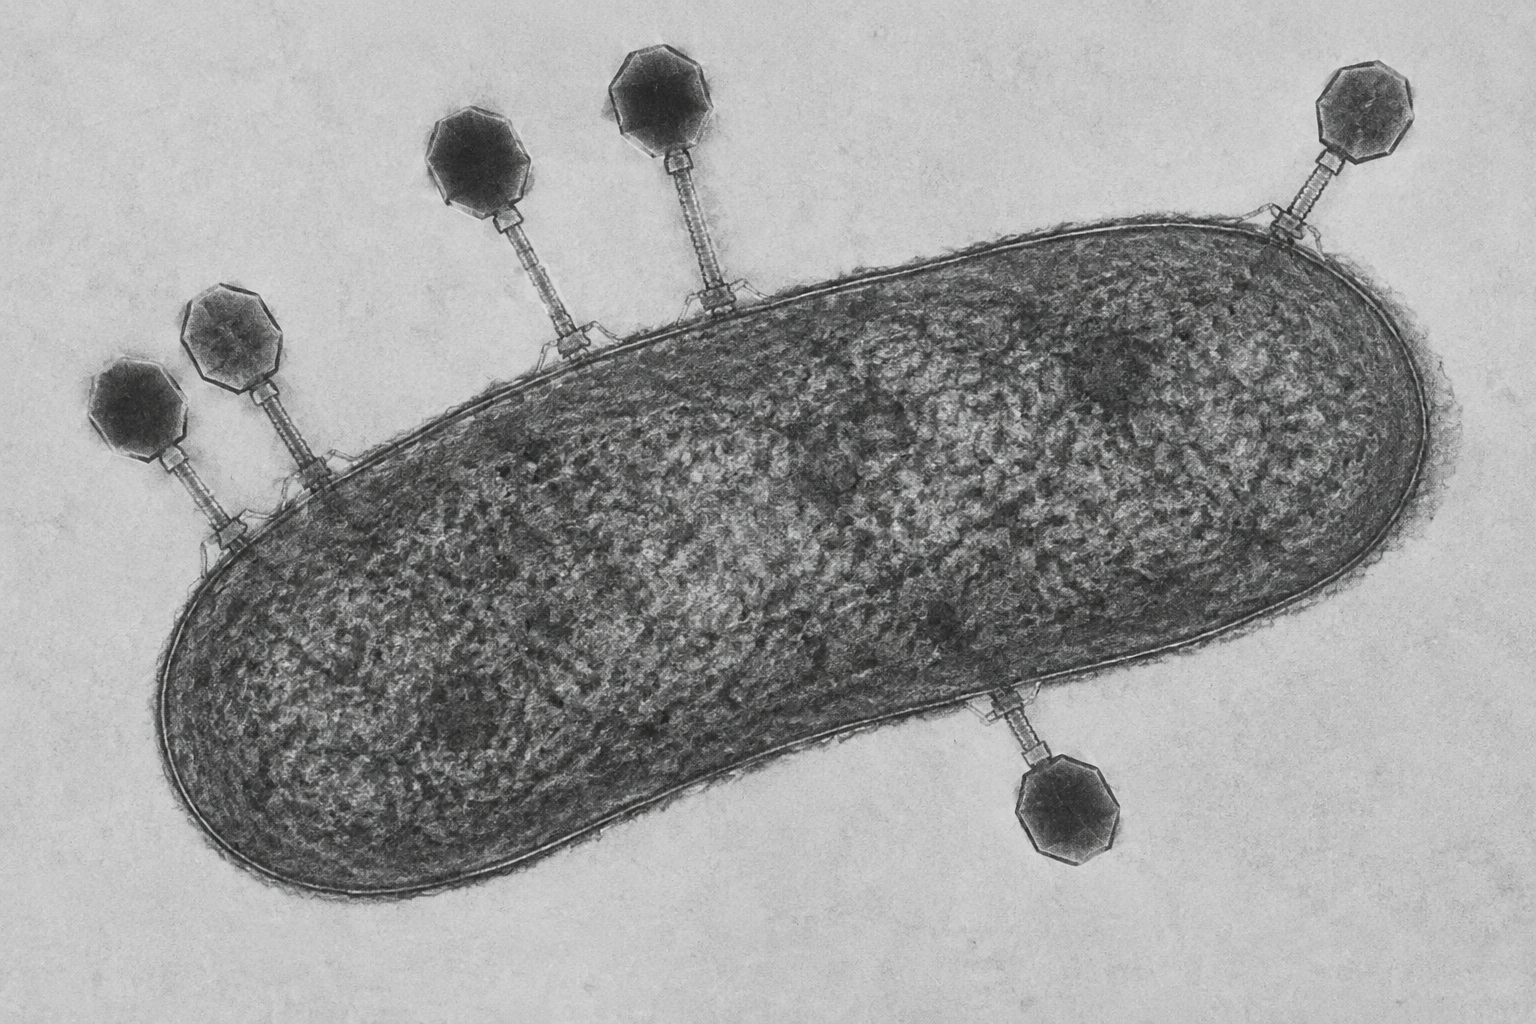
\includegraphics[width=0.5\linewidth]{images/book3/ai/b3-17-phage-on-bacterium.png}

{\small Bacteriófagos presos a uma bactéria: cabeças poliédricas que
contêm o \omterm{def:b1:nucleic-acids:chain}{DNA}, e caudas pelas quais ele será injetado. Uma única \omterm{def:b1:cell-unit-of-life:cell}{célula}
liberará uma centena de fagos novos em meia hora.}
\end{omfigure}

\begin{proposition}[Os dois ciclos do fago $\lambda$]\label{prop:b1:genomes:lambda}
\index{ciclo lítico}\index{ciclo lisogênico}
O fago $\lambda$ injeta os \qty{48.5}{kb} de \omterm{def:b1:nucleic-acids:chain}{DNA} dele
(\cref{ch:b1:nucleic-acids}) na \emph{E. coli}, onde ele se
circulariza. Dois destinos se seguem. No \emph{\omterm{prop:b1:genomes:lambda}{ciclo lítico}} os \omterm{def:b1:genomes:gene}{genes} do
fago são transcritos pela polimerase do hospedeiro, o \omterm{def:b1:nucleic-acids:chain}{DNA} dele é
replicado cem vezes, as \omterm{def:b1:proteins:peptide}{proteínas} do \omterm{def:b1:genomes:virus}{capsídeo} são fabricadas e montadas,
o \omterm{def:b1:nucleic-acids:chain}{DNA} é empacotado nelas, e uma \omterm{def:b1:enzymes:enzyme}{enzima} dissolve a parede: a \omterm{def:b1:cell-unit-of-life:cell}{célula}
estoura, liberando uma centena de fagos, quarenta minutos depois da
infecção. No \emph{\omterm{prop:b1:genomes:lambda}{ciclo lisogênico}} o \omterm{def:b1:nucleic-acids:chain}{DNA} do fago é inserido no
\omterm{def:b1:genomes:genome}{cromossomo} do hospedeiro e silenciado por um repressor de fabricação
própria: o \emph{prófago} é copiado junto com o \omterm{def:b1:genomes:genome}{cromossomo} por gerações,
invisível, até que um dano ao \omterm{def:b1:nucleic-acids:chain}{DNA} do hospedeiro suspenda a repressão e o
\omterm{prop:b1:genomes:lambda}{ciclo lítico} recomece. A escolha é um interruptor molecular, um dos
primeiros que se compreenderam (\cref{ch:b1:expression-control}).
\end{proposition}

\begin{omfigure}
\begin{tikzpicture}[font=\footnotesize, >=Stealth, line cap=round,
  st/.style={draw, thick, rounded corners=3pt, inner sep=3pt, align=center, fill=white}]
  \node[st, fill=omDef!12] (inj) at (0,0) {DNA do fago injetado,\\ circularizado};
  \node[st, fill=omThm!12] (rep) at (4.6,1.4) {replicação, proteínas\\ do capsídeo, montagem};
  \node[st, fill=omThm!12] (lys) at (9.2,1.4) {lise: \qty{100}{} fagos\\ liberados, \qty{40}{min}};
  \node[st, fill=omExo!12] (pro) at (4.6,-1.4) {integrado como prófago,\\ silenciado pelo repressor dele};
  \node[st, fill=omExo!12] (div) at (9.2,-1.4) {copiado com o cromossomo\\ do hospedeiro por gerações};
  \draw[->, thick, omThm] (inj) -- (rep) node[pos=0.45, above left, omThm] {lítico};
  \draw[->, thick, omThm] (rep) -- (lys);
  \draw[->, thick, omExo!70!black] (inj) -- (pro) node[pos=0.4, below left, omExo!70!black] {lisogênico};
  \draw[->, thick, omExo!70!black] (pro) -- (div);
  \draw[->, thick, dashed, gray] (div.north) -- (lys.south) node[midway, right, align=left, font=\scriptsize] {indução\\ (DNA do hospedeiro danificado)};
\end{tikzpicture}

{\small O fago $\lambda$: \omterm{prop:b1:genomes:lambda}{ciclo lítico} (vermelho) ou lisogênico (verde),
e a indução que transforma o segundo no primeiro.}
\end{omfigure}

\begin{example}[Vírus com genomas de RNA]\label{ex:b1:genomes:rna}
O \omterm{def:b1:genomes:virus}{vírus} da gripe carrega oito segmentos de \omterm{def:b1:nucleic-acids:chain}{RNA} de fita simples e uma
polimerase própria para copiá-los, já que as \omterm{def:b1:cell-unit-of-life:cell}{células} não têm \omterm{def:b1:enzymes:enzyme}{enzima} que
copie \omterm{def:b1:nucleic-acids:chain}{RNA}; a polimerase dele comete um erro a cada \num{10000} bases e o
\omterm{def:b1:genomes:virus}{vírus} muda a cada temporada. Um retrovírus (o HIV) carrega \omterm{def:b1:nucleic-acids:chain}{RNA} e uma
\emph{transcriptase reversa} que o copia em \omterm{def:b1:nucleic-acids:chain}{DNA}, que é inserido no
\omterm{def:b1:genomes:genome}{cromossomo} do hospedeiro como um prófago --- uma infecção permanente. Os
mecanismos, e a resposta imune a eles, são do volume do Ano 3; aqui eles
marcam a amplitude do que um \omterm{def:b1:genomes:genome}{genoma} pode ser.
\end{example}

\section{Exercícios}

\begin{exercise}[$\star$]\label{exo:b1:genomes:1}
Compare o \omterm{def:b1:genomes:genome}{genoma} bacteriano com o eucariótico: número e forma dos
\omterm{def:b1:genomes:genome}{cromossomos}, localização, \omterm{def:b1:proteins:peptide}{proteínas} que os organizam e densidade de
\omterm{def:b1:genomes:gene}{genes}.
\end{exercise}

\begin{exercise}[$\star$]\label{exo:b1:genomes:2}
Descreva um \omterm{def:b1:genomes:nucleosome}{nucleossomo} e dê o fator de compactação de cada nível de
dobramento da \omterm{def:b1:genomes:nucleosome}{cromatina}.
\end{exercise}

\begin{exercise}[$\star$]\label{exo:b1:genomes:3}
A partir da figura do censo, que fração do \omterm{def:b1:genomes:genome}{genoma} humano codifica
\omterm{def:b1:proteins:peptide}{proteína}, e qual é a maior categoria?
\end{exercise}

\begin{exercise}[$\star$]\label{exo:b1:genomes:4}
O que é um \omterm{def:b1:genomes:virus}{vírus}, e em que sentido ele não é vivo?
\end{exercise}

\begin{exercise}[$\star\star$]\label{exo:b1:genomes:5}
Calcule o comprimento do \omterm{def:b1:genomes:genome}{cromossomo} da \emph{E. coli} e o número de
voltas do tamanho de um \omterm{def:b1:genomes:nucleosome}{nucleossomo} de que ele precisaria se fosse
eucariótico; explique como a bactéria o compacta em vez disso.
\end{exercise}

\begin{exercise}[$\star\star$]\label{exo:b1:genomes:6}
Um \omterm{def:b1:genomes:gene}{gene} humano de \qty{27}{kb} tem \qty{1.5}{kb} de \omterm{def:b1:genomes:gene}{éxons} em oito
pedaços. Calcule os comprimentos médios de \omterm{def:b1:genomes:gene}{éxon} e de \omterm{def:b1:genomes:gene}{íntron} e a fração
do transcrito primário que é descartada.
\end{exercise}

\begin{exercise}[$\star\star$]\label{exo:b1:genomes:7}
Usando a tabela, calcule os \omterm{def:b1:genomes:gene}{genes} por megabase da \emph{E. coli}, da
levedura, da mosca-das-frutas, do ser humano e do peixe pulmonado.
Comente a tendência.
\end{exercise}

\begin{exercise}[$\star\star$]\label{exo:b1:genomes:8}
O elemento Alu tem \qty{300}{bp} e está presente em um milhão de cópias.
Que fração do \omterm{def:b1:genomes:genome}{genoma} é Alu? Se cada cópia tiver surgido por
retrotransposição (um \omterm{def:b1:nucleic-acids:chain}{RNA} copiado de volta a \omterm{def:b1:nucleic-acids:chain}{DNA} e inserido), quantas
inserções por geração produziriam um milhão de cópias em \num{60}
milhões de anos, a \num{20} anos por geração?
\end{exercise}

\begin{exercise}[$\star\star$]\label{exo:b1:genomes:9}
Explique por que o \omterm{def:b1:genomes:genome}{genoma} mitocondrial é herdado por via materna, e o
que isso implica para o rastreamento de ancestralidade.
\end{exercise}

\begin{exercise}[$\star\star\star$]\label{exo:b1:genomes:10}
O fago $\lambda$ no estado lisogênico é copiado uma vez por geração do
hospedeiro; no estado lítico ele faz cem cópias em \qty{40}{min}. Numa
cultura bem alimentada que dobra a cada \qty{20}{min}, compare as duas
estratégias ao longo de duas horas; numa cultura em inanição que não se
divide, compare-as de novo. Por que o interruptor responde à condição do
hospedeiro?
\end{exercise}

\begin{exercise}[$\star\star\star$]\label{exo:b1:genomes:11}
Uma \omterm{def:b1:cell-unit-of-life:cell}{célula} de peixe pulmonado carrega \qty{130}{Gb}: calcule o
comprimento do \omterm{def:b1:nucleic-acids:chain}{DNA}, o número de \omterm{def:b1:genomes:nucleosome}{nucleossomos} e a massa de \omterm{def:b1:genomes:nucleosome}{histonas} por
\omterm{def:b1:cell-unit-of-life:cell}{célula}, e o tempo para replicá-lo na velocidade humana de forquilha
(\qty{50}{bp/s} por forquilha) com uma origem a cada \qty{100}{kb}. O
que um \omterm{def:b1:genomes:genome}{genoma} grande custa a uma \omterm{def:b1:cell-unit-of-life:cell}{célula}?
\end{exercise}

\begin{exercise}[$\star\star\star$]\label{exo:b1:genomes:12}
``O \omterm{def:b1:genomes:genome}{genoma} é um registro, e não um projeto.'' Discuta em um parágrafo,
com os pseudogenes, os elementos transponíveis, as famílias gênicas e o
paradoxo do valor C.
\end{exercise}

\section{Problema: Dois metros em seis micrômetros}

\begin{problem}[{Problema de fim de semana --- um núcleo humano medido
da hélice ao cromossomo: comprimentos, volumes, nucleossomos, histonas e
a razão de empacotamento em cada nível, terminando na compactação total
da metáfase}]
\label{pb:b1:genomes:1}
Um núcleo humano diploide é uma esfera de \qty{6}{\micro m} de diâmetro
que contém $\num{6.4e9}$ \omterm{thm:b1:nucleic-acids:helix}{pares de bases} em 46 \omterm{def:b1:genomes:genome}{cromossomos}; o maior
\omterm{def:b1:genomes:genome}{cromossomo} carrega \qty{250}{Mb}, e o menor \qty{50}{}. Tome
\qty{0.34}{nm} por par, \qty{2}{nm} para o diâmetro da hélice,
\qty{650}{Da} por par, \num{200} pares por \omterm{def:b1:genomes:nucleosome}{nucleossomo}, um octâmero de
\omterm{def:b1:genomes:nucleosome}{histonas} de \qty{108}{kDa}, e $\qty{1.66e-24}{g}$ por dálton.

\medskip
\noindent\textbf{Parte I --- Comprimentos e volumes.}
\begin{enumerate}
  \item Calcule o comprimento total de \omterm{def:b1:nucleic-acids:chain}{DNA} do núcleo.
  \item Calcule o número de voltas da dupla-hélice que ele contém.
  \item Calcule o comprimento do \omterm{def:b1:nucleic-acids:chain}{DNA} do maior e do menor \omterm{def:b1:genomes:genome}{cromossomo}.
  \item Calcule o volume do núcleo.
  \item Calcule o volume do \omterm{def:b1:nucleic-acids:chain}{DNA} como um cilindro, e a fração do núcleo
        que ele ocupa.
  \item Calcule a massa de \omterm{def:b1:nucleic-acids:chain}{DNA} do núcleo em picogramas.
  \item O núcleo contém cerca de \qty{25}{pg} de \omterm{def:b1:proteins:peptide}{proteína}. Que fração da
        massa nuclear é \omterm{def:b1:nucleic-acids:chain}{DNA}, se a água for \qty{80}{\%} do núcleo
        (densidade \qty{1.1}{g/mL})?
\end{enumerate}

\medskip
\noindent\textbf{Parte II --- \omterm{def:b1:genomes:nucleosome}{Nucleossomos}.}
\begin{enumerate}[resume]
  \item Calcule o número de \omterm{def:b1:genomes:nucleosome}{nucleossomos} do núcleo.
  \item Calcule a massa das \omterm{def:b1:genomes:nucleosome}{histonas} e compare com a massa de \omterm{def:b1:nucleic-acids:chain}{DNA}.
  \item Os \qty{200}{} pares de um \omterm{def:b1:genomes:nucleosome}{nucleossomo} abrangem \qty{68}{nm} de
        hélice, mas ocupam uma conta de \qty{11}{nm} de comprimento.
        Calcule o fator de compactação das ``contas num colar''.
  \item A fibra de \qty{30}{nm} contém seis \omterm{def:b1:genomes:nucleosome}{nucleossomos} por
        \qty{11}{nm} de comprimento dela. Calcule o fator de compactação
        dela em relação ao \omterm{def:b1:nucleic-acids:chain}{DNA} nu.
  \item Calcule o comprimento da fibra de \qty{30}{nm} para o \omterm{def:b1:genomes:genome}{genoma}
        inteiro, e compare-o com o diâmetro do núcleo.
  \item Cada \omterm{def:b1:genomes:nucleosome}{nucleossomo} precisa ser desmontado e remontado quando o \omterm{def:b1:nucleic-acids:chain}{DNA}
        é replicado ou transcrito. Quantos \omterm{def:b1:genomes:nucleosome}{nucleossomos} são remontados
        na fase S (\qty{8}{h})? E por segundo?
\end{enumerate}

\medskip
\noindent\textbf{Parte III --- Alças e \omterm{def:b1:genomes:genome}{cromossomos}.}
\begin{enumerate}[resume]
  \item Alças de \qty{75}{kb} da fibra de \qty{30}{nm} pendem de um
        arcabouço. Calcule o comprimento de fibra de uma alça e o número
        de alças do \omterm{def:b1:genomes:genome}{genoma}.
  \item Uma cromátide metafásica do maior \omterm{def:b1:genomes:genome}{cromossomo} tem
        \qty{10}{\micro m} de comprimento. Calcule o fator de
        compactação do \omterm{def:b1:nucleic-acids:chain}{DNA} nu ao \omterm{def:b1:genomes:genome}{cromossomo} metafásico.
  \item Calcule o volume dessa cromátide como um cilindro de
        \qty{0.7}{\micro m} de diâmetro, e a fração dele que é \omterm{def:b1:nucleic-acids:chain}{DNA}.
  \item Os 46 \omterm{def:b1:genomes:genome}{cromossomos} na metáfase, cada um um bastão da mesma
        densidade: calcule o volume total deles e compare com o do
        núcleo interfásico.
  \item Explique por que a \omterm{def:b1:genomes:nucleosome}{cromatina} interfásica não pode ser empacotada
        tão apertada quanto a metafásica.
\end{enumerate}

\medskip
\noindent\textbf{Parte IV --- Encontrar um \omterm{def:b1:genomes:gene}{gene}.}
\begin{enumerate}[resume]
  \item Uma \omterm{def:b1:proteins:peptide}{proteína} precisa encontrar um sítio de \qty{20}{bp} no
        \omterm{def:b1:genomes:genome}{genoma}. Se ela testasse um sítio ao acaso por milissegundo,
        quanto tempo levaria a busca? O que isso diz sobre como os
        sítios são encontrados?
  \item Os \qty{20000}{} \omterm{def:b1:genomes:gene}{genes} do \omterm{def:b1:genomes:genome}{genoma} têm em média \qty{27}{kb}. Que
        fração do \omterm{def:b1:genomes:genome}{genoma} está dentro de \omterm{def:b1:genomes:gene}{genes}? Que fração é
        codificante, a \qty{1.5}{kb} de \omterm{def:b1:genomes:gene}{éxons} por \omterm{def:b1:genomes:gene}{gene}?
  \item Cada \omterm{def:b1:genomes:genome}{cromossomo} ocupa um território próprio no núcleo. Calcule o
        volume do território do maior \omterm{def:b1:genomes:genome}{cromossomo}, se os territórios
        forem proporcionais ao conteúdo de \omterm{def:b1:nucleic-acids:chain}{DNA}, e a concentração de \omterm{def:b1:nucleic-acids:chain}{DNA}
        dentro dele, em \omterm{thm:b1:nucleic-acids:helix}{pares de bases} por micrômetro cúbico.
  \item Um núcleo de peixe pulmonado com a mesma densidade de \omterm{def:b1:nucleic-acids:chain}{DNA} teria
        que volume para \qty{260}{Gb} (em diploidia)? E que diâmetro?
  \item Calcule o número de octâmeros de \omterm{def:b1:genomes:nucleosome}{histonas} que uma \omterm{def:b1:cell-unit-of-life:cell}{célula} precisa
        fabricar na fase S e os \omterm{def:b1:proteins:aminoacid}{aminoácidos} que eles contêm
        (\qty{1000}{} resíduos por octâmero). Compare com os
        \qty{3e9}{} resíduos de \omterm{def:b1:proteins:peptide}{proteína} que uma \omterm{def:b1:cell-unit-of-life:cell}{célula} fabrica por dia.
  \item Explique em duas frases por que as bactérias conseguem passar
        sem \omterm{def:b1:genomes:nucleosome}{nucleossomos} e os eucariotos não.
  \item Enuncie o resultado: o fator de compactação total da hélice ao
        \omterm{def:b1:genomes:genome}{cromossomo} metafásico, e os fatores de cada nível.
\end{enumerate}
\end{problem}
